\documentclass[12pt]{article}
\setcounter{secnumdepth}{0}
\usepackage[margin=1in]{geometry} 
\usepackage{amsmath,amsthm,amssymb}
 
\usepackage{listings}
\usepackage{color}
\usepackage{advdate}
\definecolor{dkgreen}{rgb}{0,0.6,0}
\definecolor{gray}{rgb}{0.5,0.5,0.5}
\definecolor{mauve}{rgb}{0.58,0,0.82}
\usepackage{graphicx}
\lstset{frame=tb,
  aboveskip=3mm,
  belowskip=3mm,
  showstringspaces=false,
  columns=flexible,
  basicstyle={\small\ttfamily},
  numbers=none,
  numberstyle=\tiny\color{gray},
  keywordstyle=\color{blue},
  commentstyle=\color{dkgreen},
  stringstyle=\color{mauve},
  breaklines=true,
  breakatwhitespace=true,
  tabsize=3,
  emph={  
    enterCS,
    releaseCS,
    haveResource
    },
  emphstyle={\color{dkgreen}\bfseries}
}
\begin{document}
\title{CS3563: DBMS II\\Assignment 2}
\author{Sagar Jain\\CS17BTECH11034}
\date{\AdvanceDate[-1]\today}
\maketitle
\section{Solutions}
\begin{enumerate}
\item \begin{enumerate}
\item Let,\\
S = Suppliers,\\
P = Parts,\\
C = Catalog\\

The given relational algebra query will yield the desired result:
\begin{center}
$ \Pi_{sid}(S) - \Pi_{sid}(\Pi_{sid, pid}(S * \Pi_{pid}(\sigma_{colour=blue}(P))) - \Pi_{sid, pid}(C)) $
\end{center}
\item The given SQL query will yield the required result:\\\\
\texttt{SELECT sid, min(price) FROM Catalog NATURAL JOIN Suppliers GROUP BY sid HAVING COUNT (DISTINCT pid) > 1;}\\

\item The following domain relational calculus query will yield the required result:\\\\
$ \{ \langle sname,\,colour \rangle \; | \; \exists \; sid,address \; \langle sid,\; sname,\; address\rangle \in Suppliers \; \land \; \exists \; pid, pname \\\; \langle pid, \;pname, color \rangle \in Parts  \land  \exists \; price\; \langle sid,\;pid,\; price \rangle \; \in Catalog \} $\\
\item A query of the following form would not be possible in plain SQL:\\
\texttt{Given a string s, list all the combinations of sids and or pids which can be concatenated to form s.} 
\end{enumerate}
\item F2: $CD \rightarrow ABF $\\
F1 and F2 together result in BCNF because the lhs of both are superkeys and F2 cannot be logically inferred from F1.\\
F3: $BF \rightarrow C $\\
C belongs to a candidate key, BF are not a superkey and the dependency cannot be logically inferred from F1. So F1, F2, F3 result in 3NF.
\item 
\begin{enumerate}
\item ER Diagram:\\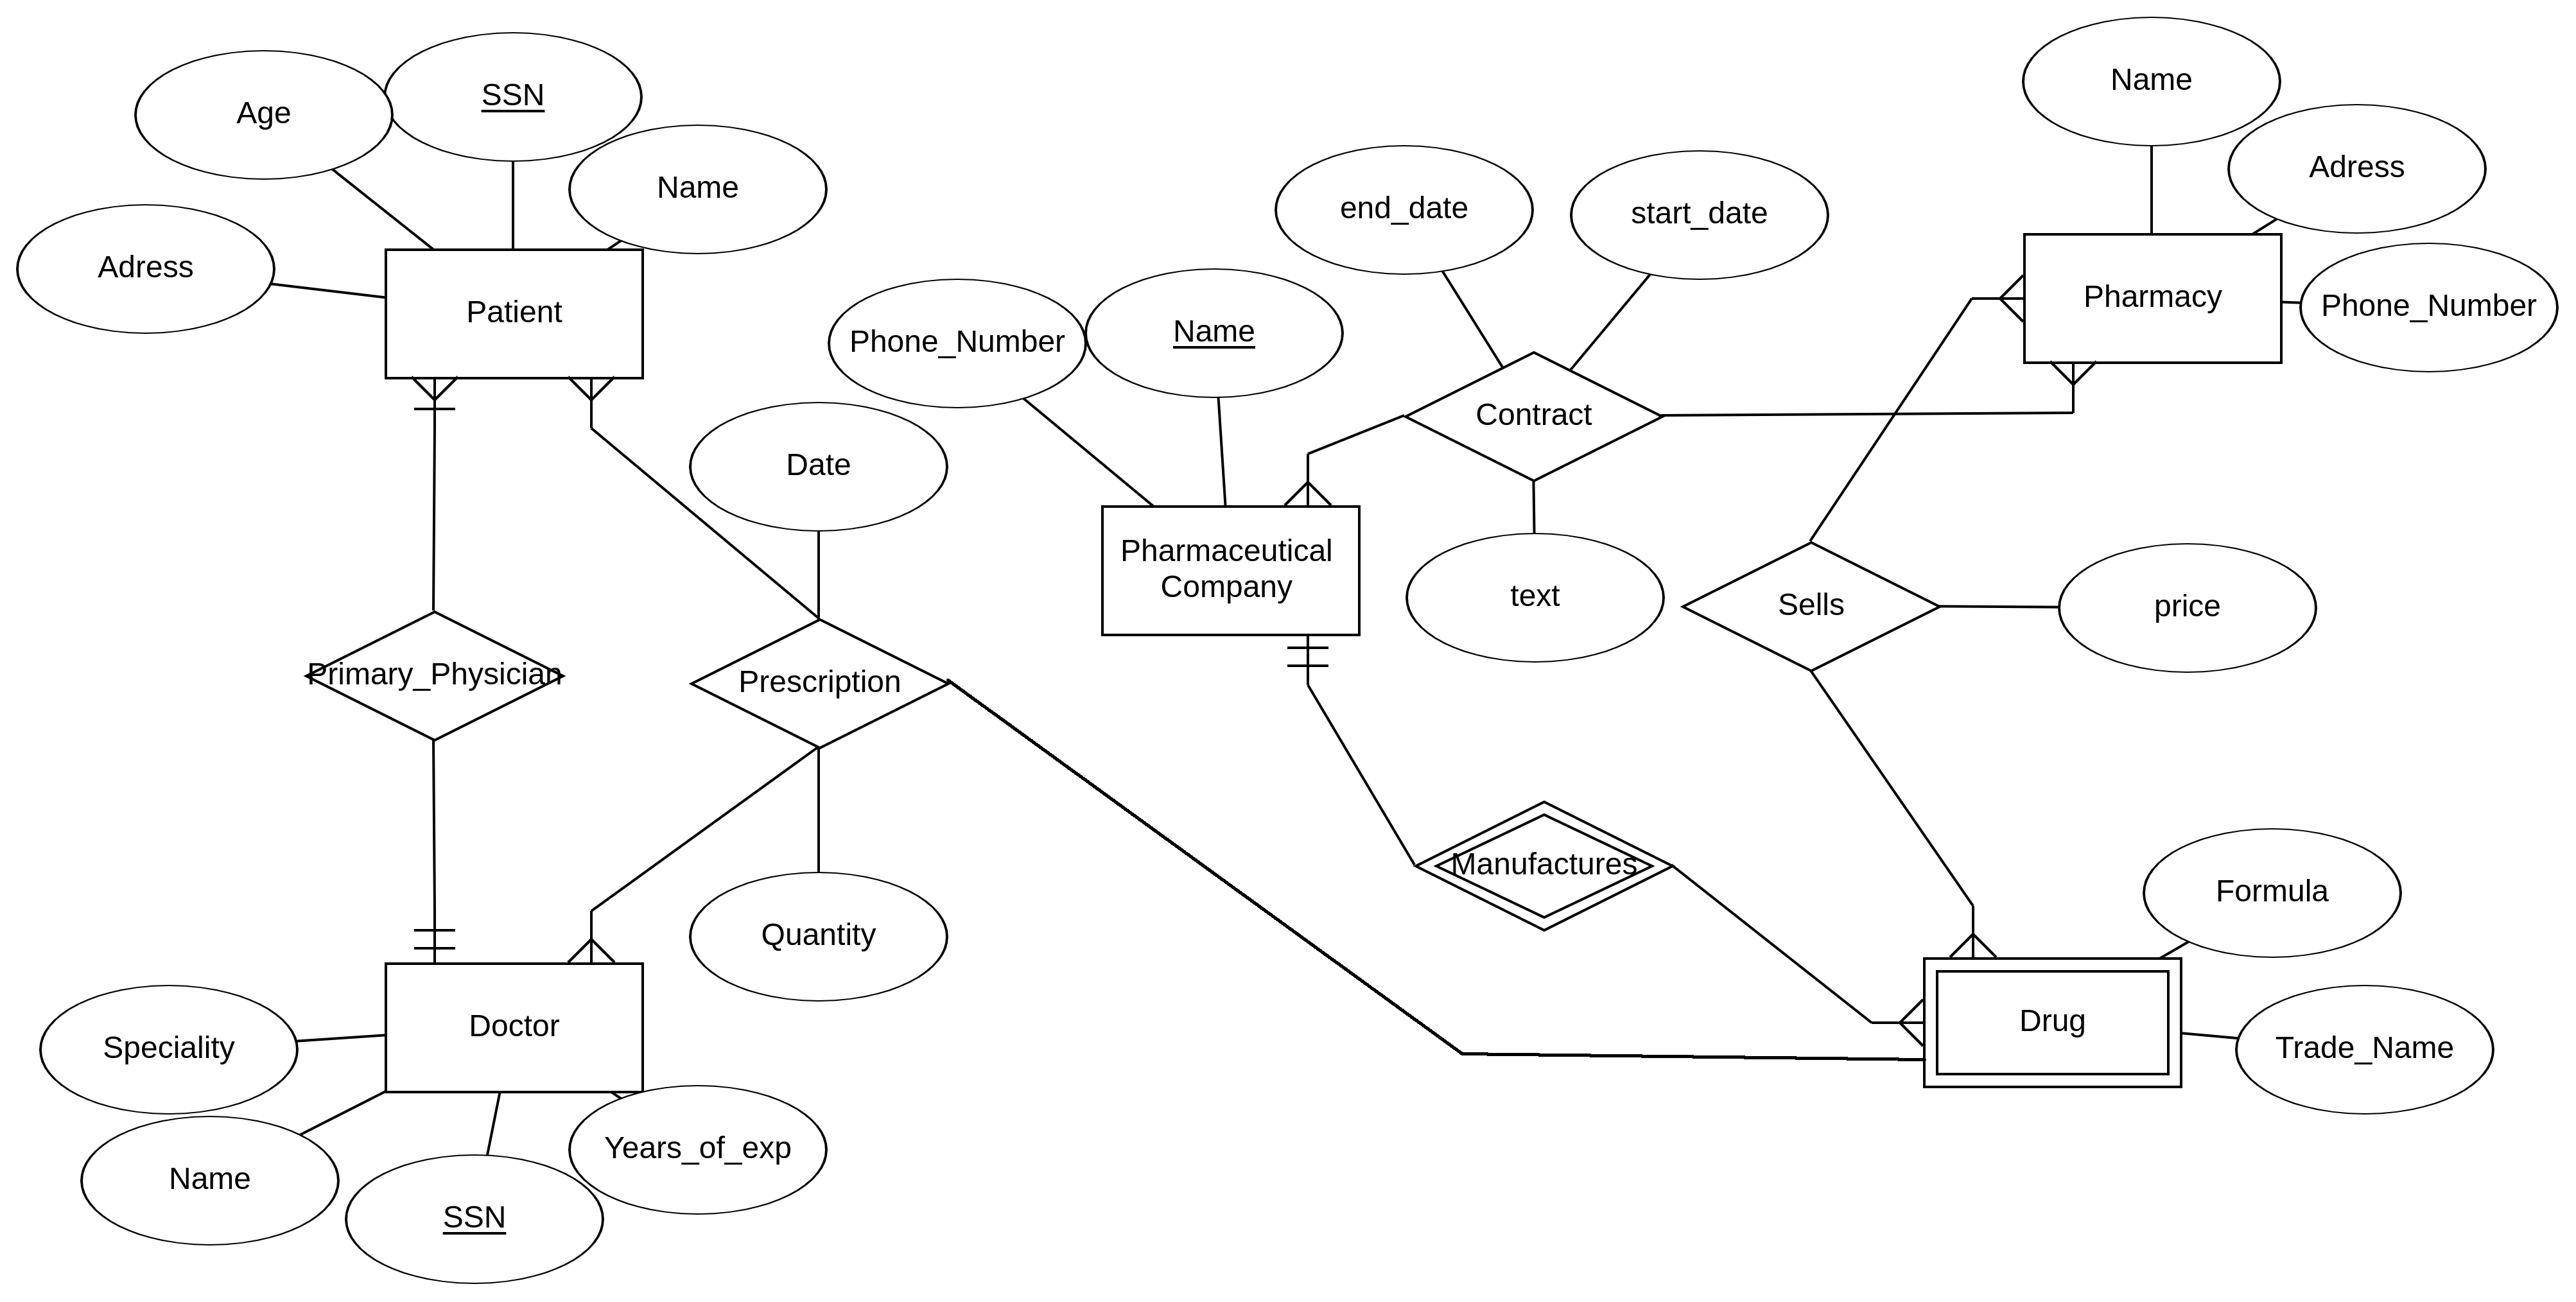
\includegraphics[scale=0.12]{erd.png}
\item There would be no problem in storing multiple prescriptions in the current model except when there are two prescriptions for the same drug on the same day and the same quantity. So we need to be able to store duplicates, for this we should make the attributes \textbf{multivalued}, but we also need to make sure that they are in the same table so they also need to be \textbf{composite}.
\end{enumerate}
\end{enumerate}
\end{document}